% Разбиение подматрицы на четыре компоненты: top/left/right/bottomSubmatrix.
% n=10, a=4, b=6, s=3. Координаты: P(i,j) = ((i+j)/2, (j-i)/2).
% Четверти разделены срединными линиями квадрата i = a-s/2 и j = b+s/2
% (в повёрнутом виде -- от середины стороны к середине противоположной).
% Цвета -- полупрозрачные заливки оригинального изображения, скомпозитированные
% на белый фон (крест -- на заливку ромба).
\definecolor{InnerTeal}{HTML}{9cc4ce}
\definecolor{InnerCross}{HTML}{f71011}

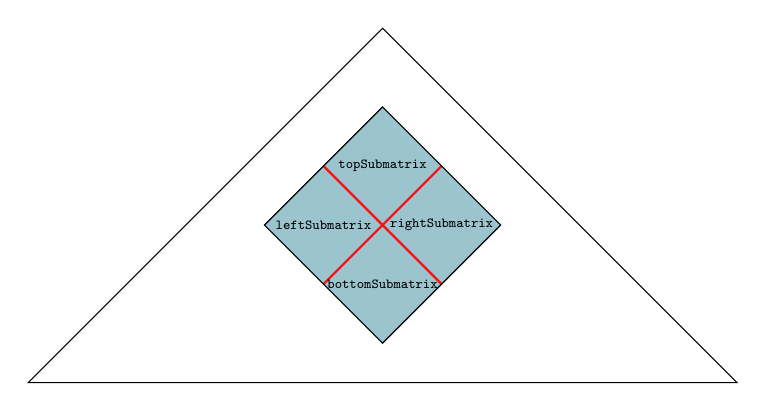
\begin{tikzpicture}
  % Треугольник таблицы
  \coordinate (BL)  at (0.5,0.5);
  \coordinate (TOP) at (5,5);
  \coordinate (BR)  at (9.5,0.5);

  % Ромб подматрицы: левый P(a-s,b), нижний P(a,b), правый P(a,b+s), верхний P(a-s,b+s)
  \coordinate (dmL) at (3.5,2.5);
  \coordinate (dmB) at (5,1);
  \coordinate (dmR) at (6.5,2.5);
  \coordinate (dmT) at (5,4);

  % Концы срединных линий (середины сторон ромба)
  \coordinate (mB) at (4.25,1.75); % i=a-s/2 на стороне j=b
  \coordinate (mT) at (5.75,3.25); % i=a-s/2 на стороне j=b+s
  \coordinate (mL) at (4.25,3.25); % j=b+s/2 на стороне i=a-s
  \coordinate (mR) at (5.75,1.75); % j=b+s/2 на стороне i=a

  % Закраска
  \fill[InnerTeal] (dmL) -- (dmB) -- (dmR) -- (dmT) -- cycle;

  % Срединные линии
  \draw[InnerCross, thick] (mB) -- (mT);
  \draw[InnerCross, thick] (mL) -- (mR);

  % Контур
  \draw (BL) -- (TOP) -- (BR) -- cycle;
  \draw (dmL) -- (dmB) -- (dmR) -- (dmT) -- cycle;

  % Подписи четвертей (мелкий шрифт, чтобы влезали в четверти-ромбики)
  \node[font=\fontsize{4pt}{4pt}\selectfont] at (5,3.25)   {\texttt{topSubmatrix}};
  \node[font=\fontsize{4pt}{4pt}\selectfont] at (4.25,2.5) {\texttt{leftSubmatrix}};
  \node[font=\fontsize{4pt}{4pt}\selectfont] at (5.75,2.5) {\texttt{rightSubmatrix}};
  \node[font=\fontsize{4pt}{4pt}\selectfont] at (5,1.75)   {\texttt{bottomSubmatrix}};
\end{tikzpicture}
